\documentclass[12pt]{article}
\usepackage{graphicx}
\usepackage{eso-pic}
\usepackage{ragged2e}
\renewcommand\thepage{- \arabic{page} -}
%Logo
\newcommand\Highlight{%
	\put(0,150){%
		\parbox[b][\paperheight]{\paperwidth}{%
		\vfill
		\centering
		
\includegraphics[width=\paperwidth, height=10cm]{logo.jpg}%
		\vfill
}}}
%Swirl
\newcommand\Swirl{%
	\put(50,270){%
		\parbox[b][\paperheight]{\paperwidth}{%
		\vfill
		\centering
		
\includegraphics[width=20cm, height=20cm]{background.png}%
		\vfill
}}}
\usepackage{graphicx}
\graphicspath{{../images/}}

\AddToShipoutPicture*{\Highlight}
\AddToShipoutPictureBG{%
	\ifnum\value{page}>1
	\AtPageLowerLeft{\Swirl}%
    \fi
    }%

\begin{document}

{\fontfamily{phv}\selectfont % change phv to get new fonts for whole document
\font\myfont=cmr12 at 20pt

\begin{center}


\begin{minipage}{0.75\linewidth}


\vspace*{250pt}
\title{ \rule{\linewidth}{2pt} \\
\textbf{\normalfont\fontsize{35}{35}\scshape\selectfont IoT HomeCare System}\\
\textbf{\normalfont\fontsize{35}{35}\scshape\selectfont Testing}\\}
\author{
        Hristian Vitrychenko\\
        Nikki Constancon \\
        Juan du Preez\\
        Gregory Austin \\
        Marthinus Richter
}
\date{\today \\ \rule{\linewidth}{2pt}}


\maketitle
\thispagestyle{empty}

\end{minipage}
\end{center}
\pagebreak
	\section{Introduction}

	The testing report is designed to describe all tests that have been done on the system.

		\subsection{Purpose}

		The purpose of this document will be to list and describe all of the tests for the ReVA system, how they are carried out, what their purpose is and what subsystem and related module(s) they are related to.

		\subsection{Structure of the document}

		Each subsystem of ReVA will be addressed individually with the specific tests for each module concerned with that subsystem. The subsystems are:
		\begin{itemize}
			\item Real-Time Subsystem \\ This includes the modules: Data Collection,  Pub/Sub Server, Data Pull, and User Interface
			\item Data Storage Subsystem \\ This includes the modules: Data Storage, Pub/Sub Server
			\item History/Statistics Subsystem \\ This includes the modules: Data Storage, Statistics, Pub/Sub Server, and User Interface
			\item User Management Subsystem \\ This includes the modules: User Management, User Interface
			\item Notification Subsystem \\ This includes the modules: Pub/Sub Server, Notification, and User Interface
			\item Advice Subsystem \\ This includes the modules: Advice and User Interface
		\end{itemize}
		\subsection{Definitions, Acronyms, and Abbreviations}


			\subsubsection{Acronyms}

			\begin{itemize}

				\item \textbf{UI} \textbf{\textit{(User Interface)}} \\
				\newline
				The means by which the user and a computer system interact, in particular, the use of input devices and software.

			\end{itemize}

			\subsubsection{Definitions}

			\begin{itemize}

				\item \textbf{Unit Test}\\
				\newline
				Unit testing is a software development process in which the smallest testable parts of an application, called units, are individually and independently scrutinised for proper operation.\\
				\item \textbf{Integration Test}\\
				\newline 
				Find out if the units if integrated together will work without errors. For example, argument passing and data updation etc.
				\item \textbf{Functionality Test}\\
				\newline 
				Tests all functionalities of the software against the requirement.
				\item \textbf{Performance Test}\\
				\newline 
				This test proves how efficient the software is. It tests the effectiveness and average time taken by the software to do desired task. Performance testing is done by means of load testing and stress testing where the software is put under high user and data load under various environment conditions.
				\item \textbf{Alpha Testing}\\
				\newline 
				The team of developer themselves perform alpha testing by using the system as if it is being used in work environment. They try to find out how user would react to some action in software and how the system should respond to inputs.

			\end{itemize}

		\subsection{Additional Information}

		The code being tested is written by different developers, thus this document serves as a way in order to review the functionality and tests done, and to provide information about said tests on current functionality.\\\\


	\pagebreak

	\section{Real-time subsystem}
	\textbf{Modules involved:} Data Collection,  Pub/Sub Server, Data Pull, and User Interface \\
	\textbf{Primary Actors:} All users \\
	\textbf{Functionality:} View real time data on patient(s)\\
	\subsubsection{Description of current tests}
	The data streaming consists of Raspberry pi's streaming to servers, and servers streaming that data out and the application displaying those data streams. We do this using the Nodejs package Zetta (which is already been tested) for the Data Collection and the Pub/Sub Server, and an open source Zetta-Starter-Android-Application developed to interface with the Zetta API to recieve the streams (DataPull) that's generated by the server which has also been tested. These have all been tested individually already, thus to create our own unit tests would be redundant. \\ \\ 

	The current tests are Integration Tests to see that data is in fact streaming from and to devices. You can see the tests in the three figures below. 
	\begin{figure}[h!]
		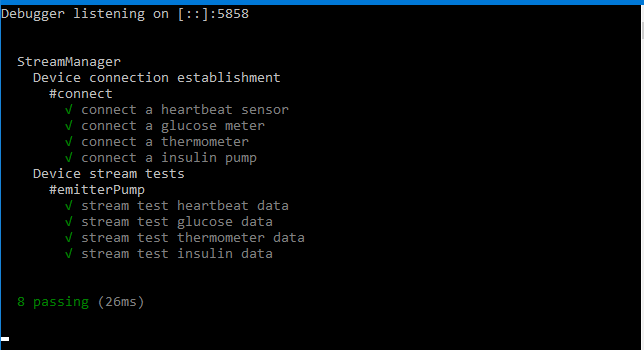
\includegraphics[width=\textwidth]{tests/zettaStream/test-zetta-stream-pass}
		\caption{Mocha output of successful mock device streams}
	\end{figure}
	\begin{figure}[h!]
		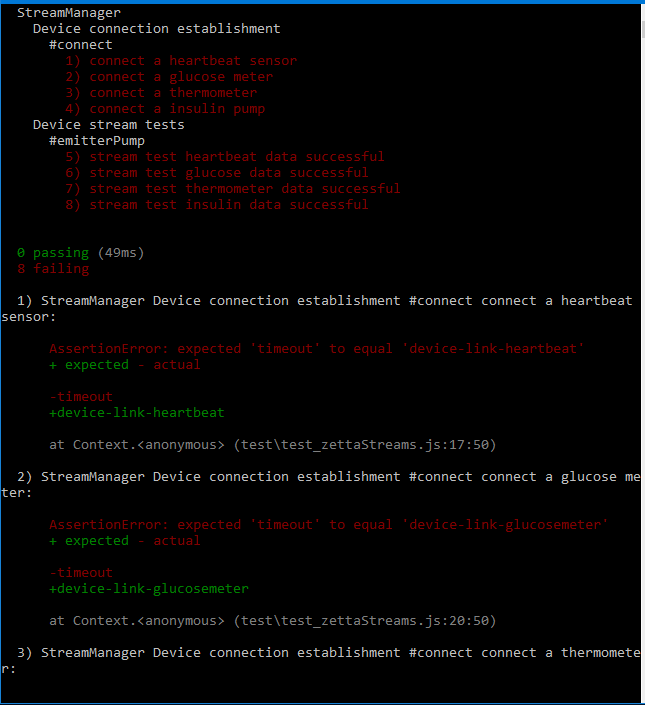
\includegraphics[width=\textwidth]{tests/zettaStream/test-zetta-stream-fail00}
		\caption{Mocha output (1 of 2) for unsuccessful mock device streams (due to being programmatic disabled)}
	\end{figure}
	\begin{figure}[h!]
	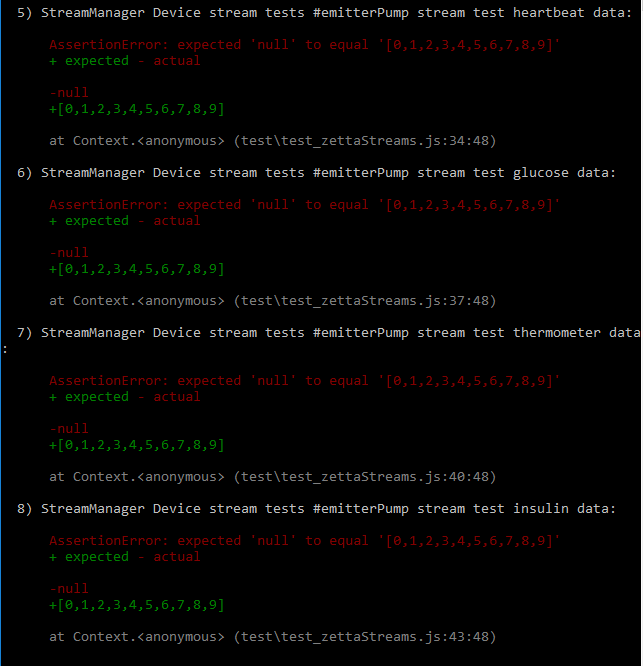
\includegraphics[width=\textwidth]{tests/zettaStream/test-zetta-stream-fail01}
	\caption{Mocha output (2 of 2) for unsuccessful mock device streams (due to being programmatic disabled)}
	\end{figure}
	\subsubsection{Alpha tests:}
	Alpha Testing (testing it ourselves to potentially find problems) has been done each time new items or functionality has been added to the server or application. This is evidence of "eating our own cooking", and we have tried many different pathways that users would try in the application in order to make sure everything is working as it should. 
	\subsubsection{Data Collection}
	\textbf{Comment:} At the moment the Pi collects data from mock devices. This data generated and streamed using the zetta architecture and therefore has already been tested with Unit tests thoroughly. (Zetta is an open source Nodejs project purposed for IoT)
	\subsubsection{Pub/Sub Server}
	\textbf{Comment:} The Pub/Sub server uses zetta architecture as well and that's how it communicates with the pi (recieves streams being published) and any requesting devices looking to subscribe. Zetta already is established and has tests.

	\subsubsection{Data Pull}
	\textbf{Comment:} The way the data is pulled is by using the architecture of the open source Zetta-Starter-Android-Application developed to interface with the Zetta API that's generated by the server. This has also been tested, so testing is redundant.
	\subsubsection{User Interface}
	\textbf{Comment:} The user interface only displays data, and therefore it is easy to verify what is being displayed and that it is working as expected.
	
	
	
	
	
	%!!!!!!!!!!!!!!!!!!!!!!!!!!!!!!!!!!!!!!!!!!!!!!!!BREAK!!!!!!!!!!!!!!!!!!!!!!!!!!!!!!!!!!!!!!!!!!!!!!!
	\pagebreak
	%!!!!!!!!!!!!!!!!!!!!!!!!!!!!!!!!!!!!!!!!!!!!!!!!BREAK!!!!!!!!!!!!!!!!!!!!!!!!!!!!!!!!!!!!!!!!!!!!!!!

	\section{Data Storage Subsystem}
	\textbf{Modules involved: } Data Storage, Pub/Sub Server \\
	\textbf{Functionality:} Persist patient's data\\
	Unit tests where executed to verify that the zetta kit was integrated seamlessly, allowing the system to pass timestamped real-time data to the associated Cassandra. Unit tests where also executed to ensure that obtained data is persisted correctly.

	\section{History/Statistics subsystem}
	\textbf{Modules involved:} Data Storage, Statistics, Pub/Sub Server, and User Interface\\
	\textbf{Functionality:} View statistical data of patient(s)\\
	Unit tests for each coupled module where executed. For statistics this included unit testing for verification of getting the right data from queries, as well as any mathematics done by the statistics module, e.g., min, max, avg, mean etc. The user-interface performed unit-testing to make sure that graphs are being shown as specified, or statistics about the patient are indeed correct. Other tests where included to test integration to make sure everything is communicating as expected. There was also be functionality testing to ensure that the History/Statistics subsystem meets the SRS accurately. 

	\section{User Management Subsystem }
	\textbf{Modules involved} User Management, User Interface


	\subsubsection{User Management}

	\textbf{Primary Actors:} users, admin users \\
	\textbf{Functionality} Create, Remove, Update or Delete items related to data storage, e.g., user info, users, user relationships etc.  \\
	\subsubsection{Description of current tests}
	\textbf{Precondition:} The user manager is tested to ensure that arguments passed to the database manager are correctly formatted, i.e., that the json conforms to the database model. \\
	\textbf{Postcondition:} Ensure that intended parameters are added to the database after successful query. \\
	\textbf{Invariant:} Ensure that only intended parameters change within the related managers and database. \\
	\textbf{Example of when the CRUD test passes}
	\begin{center}
	\begin{figure}[h!]
		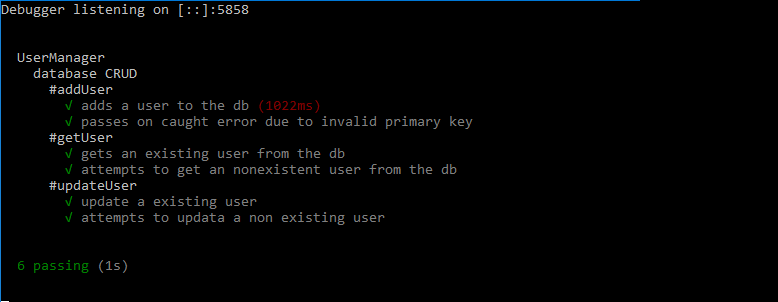
\includegraphics[width=\textwidth]{tests/usrCRUD/tests-pass.png}
		\caption{Mocha output of successful \textit{User Manager} test}
	\end{figure}
	\end{center}
	\textbf{User Manager CRUD fail example, due to Cassandra database being down. Note error reports on the console is also piped into a rotating file. Thus systems users will be able to track down errors after they occur.}
	\begin{center}
	\begin{figure}[h!]
		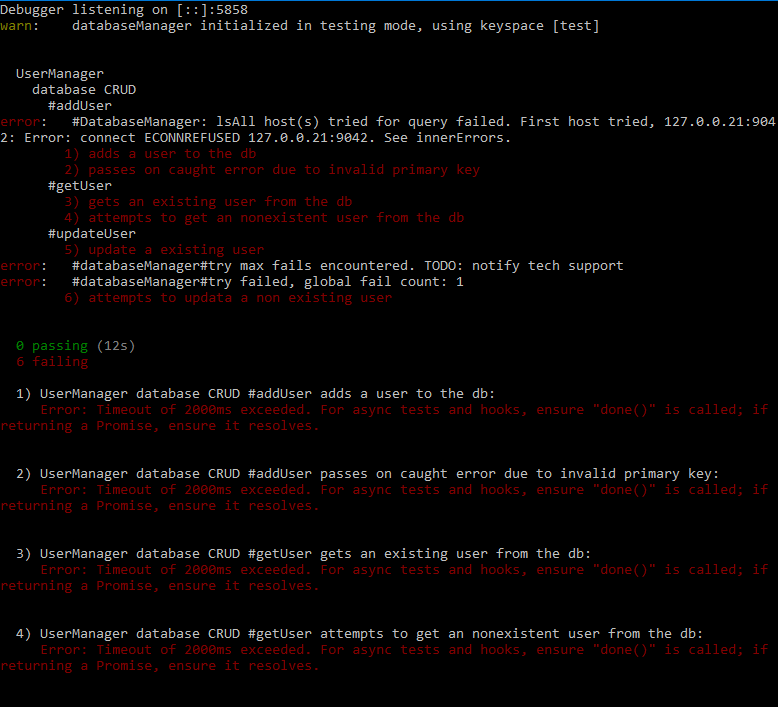
\includegraphics[width=\textwidth]{tests/usrCRUD/tests-fail.png}
		\caption{Mocha output of unsuccessful \textit{User Manager} test, due to database connection failure}
	\end{figure}
	\end{center}

%!!!!!!!!!!!!!!!!!!!!!!!!!!!!!!!!!!!!!!!!!!!!!!!!BREAK!!!!!!!!!!!!!!!!!!!!!!!!!!!!!!!!!!!!!!!!!!!!!!!
\pagebreak
%!!!!!!!!!!!!!!!!!!!!!!!!!!!!!!!!!!!!!!!!!!!!!!!!BREAK!!!!!!!!!!!!!!!!!!!!!!!!!!!!!!!!!!!!!!!!!!!!!!!

	\subsubsection{User Interface}
	\textbf{Primary Actors:} all users \\
	\textbf{Functionality} Type in details and register to become a new user. There is only local validation and forms currently implemented. Client-server communication for registration and user management is not yet implemented.
	\subsubsection{Description of current tests}
	There are unit tests for each input that test the validation of those inputs. So there are tests for email, passwords, usernames etc. All to make sure that the validation is correct. \\
	Integration tests to verify client-server communication was executed together with functionality tests to confirm the User Management subsystem adheres to the requirements. 
	\textbf{Following is the code for each unit test to show what is tested.}
	\begin{center}
	\begin{figure}[h]
		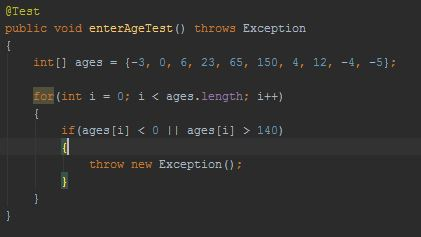
\includegraphics[width=\textwidth]{tests/usrUI/TestAge.JPG}
	\end{figure}

	\begin{figure}[h]
		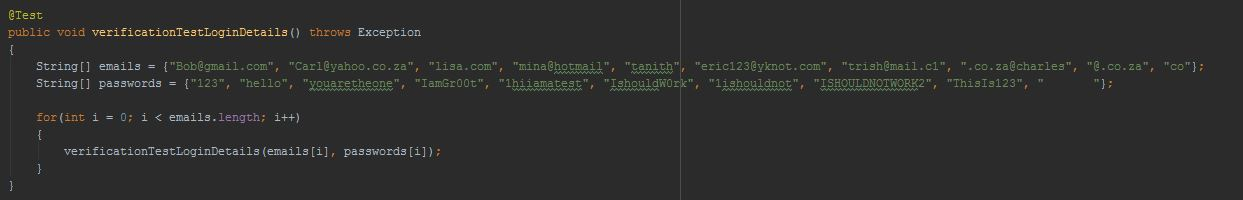
\includegraphics[width=\textwidth]{tests/usrUI/TestLogin.JPG}
	\end{figure}

	\begin{figure}[h]
		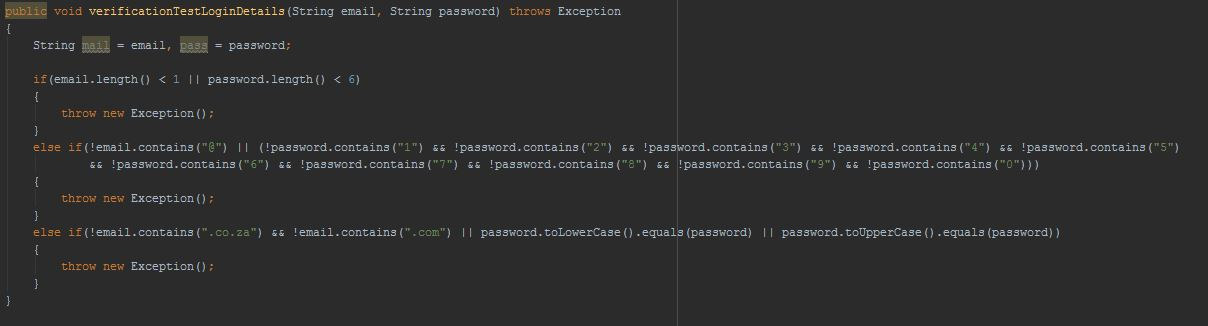
\includegraphics[width=\textwidth]{tests/usrUI/TestLoginFunction.JPG}
	\end{figure}

	\begin{figure}[h]
		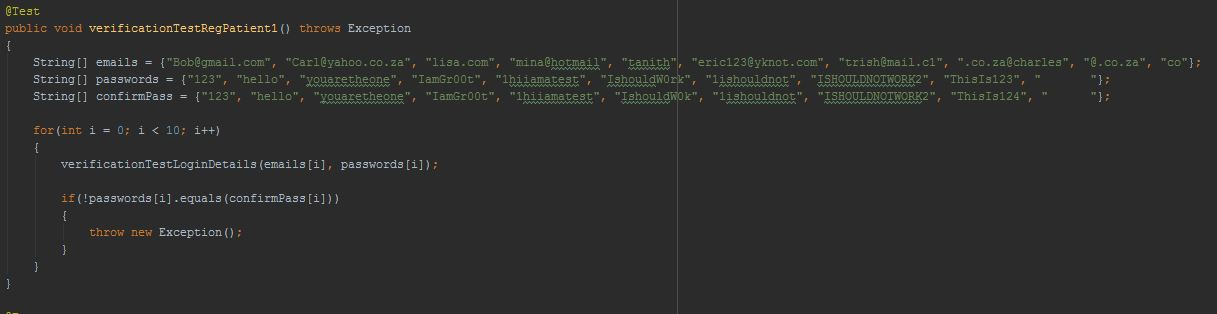
\includegraphics[width=\textwidth]{tests/usrUI/TestRegister.JPG}
	\end{figure}

	\begin{figure}[h]
		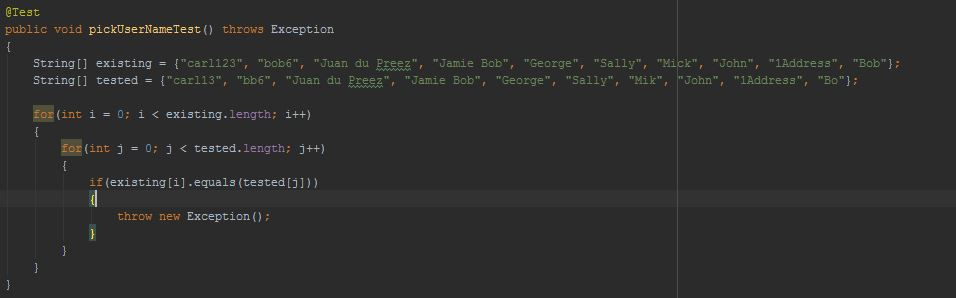
\includegraphics[width=\textwidth]{tests/usrUI/TestUsername.JPG}
	\end{figure}
	\end{center}


	\section{Notification Subsystem }
	\textbf{Modules involved:} Pub/Sub Server, Notification, and User Interface \\
	Unit tests for each individual module as well as integration tests to be sure messages are being passed properly between modules was executed. 

	\section{Tests based on non-functional requirements}
	\subsection{Usability study}
	One of the keys to accurate applicable data is that the users need to be relaxed. We planned to make the usability testing as relaxed as possible, to do this
		\begin{itemize}
		\item We had lollipops and toffees ready and waiting and as a reward for finishing the test. 
		\item Clear instructions on how to get to the usability testing location, we meet with testers outside IT and took them to the venue. 
		\item Get the user familiar with the environment.
		\item If they can't do something, make sure they know it's not their fault. 
		\item We reassure that the tests are completely confidential, and for permission to use the data generated during the test as part of our results (do this with a short consent form) 
		\item To use no terms like usability testing to keep testers at ease.
		\item Tell them how long it will take.
		\item Although acting professional, some mild humour and conversation to relax participants.
		\end{itemize} 
		We planned to not alter the test results by providing clues, suggesting directions or by reacting to things they say or do. Although taking 5 minutes for a task means the task is too hard (for our app). \\ \\
		\textbf{The results will only be as good as the people you test}, so we needed to choose people who at least, to some degree, had an interest in medical IoT and the tech. People were be asked if they were interested in the application, and because we don’t know that many people, we picked people we knew (Convenience Sampling). Using our user needs we devised scenarios to carry out. \textbf{People tend to perform more naturally if you provide them with scenarios rather than instructions} so we planned scenarios.
		\subsubsection{The script}
		Welcome, we are Loop, I’m Greg, this is Nikki, Hris,and Juan. You were chosen because you have some interest in our app. Our app ReVA helps people see vitals of bedridden or ill people and allows you to do this on the go as well as stats and alerts. You guys are here to test the app to see if it’s easy to use or terrible to use, you’re not here to be tested, you’re here to test the website. We’re aiming for accurate data on the usability of our website, so just take it easy and use it as you would at home. \\ \\
Before we begin make sure you sign the disclaimer at the top of the questionnaire. You’ll find a small task sheet with tasks you have to do, try your best for each task, but if you’re stuck for more than 5 minutes don’t hesitate to ask for help. If you do get stuck that just means the website needs improving. If you are unsure if you completed a task or not, just ask us and we’ll tell you if you did. After the tasks are done fill out the questionnaire. After you’re done with that just wait for everyone to finish and then you can leave.
\subsubsection{Process followed}
We fetched the participants from outside the IT building, one participant was missing, however this was okay as we still had 6 participants. The chosen participants weren’t old or doctors, although they weren’t perfect, data of the navigation of the UI and UI impressions was still collected. We introduced ourselves and put the participants at ease with the script and lollipops and toffees. We gave each participant a task sheet and a phone with the app. We allowed them to begin whenever they felt ready. \\ \\
The users took longer than expected. This was due to the fact that some tasks on the task sheet needed requests accepted on our side, but we were not doing that. Also some mock data for vitals wasn’t streaming either so halfway through we had to tell them to use another patient for the task. We realised this was a mistake and should’ve been prepared for it. The one application on one specific phone had some particular changes at that time so it crashed on some pages. Which was not good for consistency of the test. 

\subsubsection{Tasks performed by users} 
\begin{itemize}
	\item Task 1: \textbf{Your aunt nikki has recently been bedridden with a terminal illness, she has asked you to register for the app ReVA.} Chosen because this is a common task users have to complete. Registering for the app is essential.
\item \textbf{Task 2: Now that you’re registered aunt Nikki has asked you to add her as a patient in the app, she sent you a message with her username “nikki”.} Chosen because adding patients is imperative for the purposes of ReVA. 
\item \textbf{Task 3: You need to see how your aunt is doing, check your aunts vitals.} Chosen because patient vitals is the core requirement of the application and seeing how easy it is to navigate here is important. 
\item \textbf{Task 4: You need to see your aunts average heart rate for the last day, find out what her average heart rate is.} Chosen to see that stats is easy to navigate to and that users can easily tell where statistics is. 
\item \textbf{Task 5: Your Grampa Greg has been overcome with illness, he too asks you to add him on the app ReVA his username is ‘greg’.} Chosen so that we could see how difficult it was to change between patients and the statistics of those patients. 
\item \textbf{Task 6: Have a look at Grampa Gregs body glucose graph for the last hour and try and get a closer look at the last 15 minutes.} Chosen so that we could see that people found the graphs easy to use and intuitive to find out. 
\item \textbf{Task 7: Leave the app as you normally would, you should get a notification warning you about one of your family members. Get back to the app through the notification.} Chosen to see that alerts are intuitive and show you when there is a problem. 
\item \textbf{Task 8: Notifications have started to annoy you, turn them off.} Chosen to see that this setting was easy to find and important because not all caretakers/subscribers want or need notifications. 
\item \textbf{Task 9: Your aunt Nikki has passed away, you decide to delete her off the app reva.} Chosen for user management sake and to see that it was easy to do. 
\end{itemize}

\subsubsection{Evaluation Methods}
\textbf{Survey} \\
We used the PSSUQ because it was designed specifically for scenario-based usability studies (like ours), so some questions are more targeted, like “I was able to complete the tasks and scenarios quickly using this system.”. We used it to give us accurate data on how easy our system is to use/to navigate. The answering scale is also more complex, ranging from 1 to 7 instead of 1 to 5. This allows testers to give more nuanced responses to each question. \\
\\
The end outcome is a score from 0 to 100, reflecting the overall usability of the website or app based on the respondent’s experience. PSSUQ also has 3 sub-scores, derived from subsets of the 16 questions, which reflect system usefulness, information quality, and interface quality. System Quality (the average of items 1-6), Information Quality (the average of items 7-12), and Interface Quality (the average of items 13-16) \\
\\
\textbf{Averaged survey results} \\ 
Taking an average of the results give you a basic idea on how people perform on average. Although there can be outliers, this gives us nice easy to read data so that we can see where the problematic areas of the app are. \\ 
\\ 
\textbf{Interview with testers} \\
We did a conversational interview after everyone was done with the usability test in order to illicit any comments, criticisms or advice about the application. \\
\subsubsection{The results}
\begin{center}
	\begin{figure}[h]
		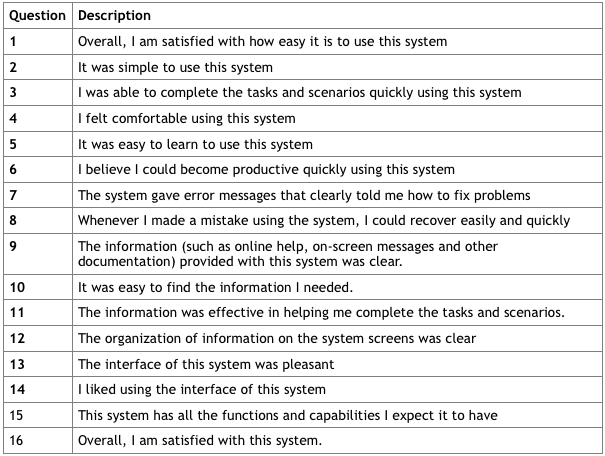
\includegraphics[width=\textwidth]{tests/usab/questions.png}
	\end{figure}
	\begin{figure}[h]
		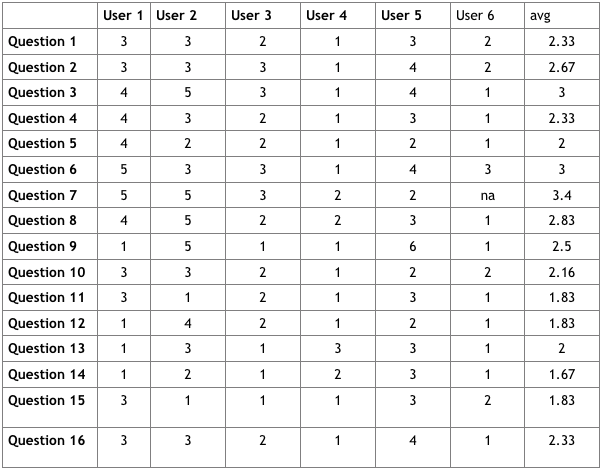
\includegraphics[width=\textwidth]{tests/usab/results.png}
	\end{figure}
	\begin{figure}[h]
		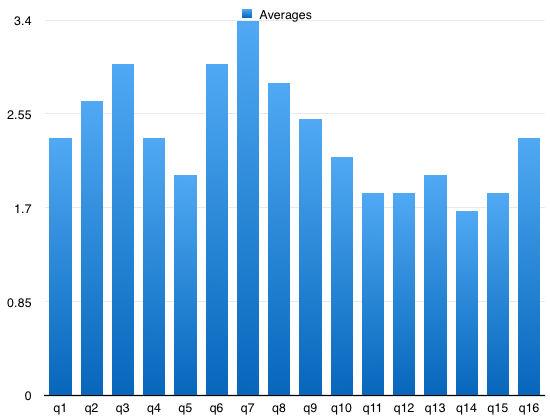
\includegraphics[width=\textwidth]{tests/usab/avgs.png}
	\end{figure}
	\begin{figure}[h]
		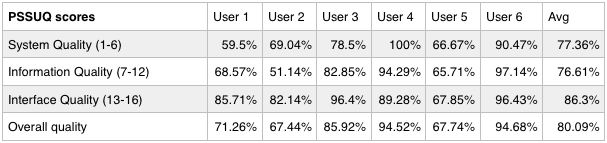
\includegraphics[width=\textwidth]{tests/usab/pssuq.png}
	\end{figure}
\end{center}

\textbf{Comments on the survey (only where there were comments)}\\
\\
\textbf{User 2 comments:}  Some serious connectivity issues on my end, but the actual functionality of the system was highly intuitive. (Maybe could be more colourful…) Also it crashed a number of times while using it (usually when loading/connecting to patient information). \\
\textbf{User 3 comments:}  Possibly a link for cellphone number for those using the app. Also medical information on where the hospital is and contact numbers linked to if there is an emergency (automatic msgs/emails) \\
\textbf{User 4 comments:} Reva stopped working when I gave the wrong password. “My connections’ had me confused when trying to add patients, but clicking it made it clear what it is. \\
\textbf{User 6 comments:} Very very nice UI and pleasant feedback when pushing buttons. Only one suggestion for enable/disable notification is have a slide lock thing just to help user’s not get confused between the enable/disable things.  \\ \\

\textbf{Results of interview with the room: } \\
There were five suggestions from the interview with the room: 
\begin{itemize}
	\item Prompt when adding a person asks for an email, but you can use username as well
	\item ‘My connections’ is a bad name for user management and should be called something like “Patient management” or “Friends management” or something
	\item Message when you’re a new user, saying what to do
	\item Refresh for the patient vitals page
	\item Partition the vitals section better so that you can easily access what you want to see
\end{itemize}	

\subsubsection{Conclusions}
Looking at the PSSUQ scores, the highest score was for the interface, however we got some lower scores for system quality and information quality. Looking at some of the lowest avg scores for some questions you can see that 3,6,7,8 are all the lowest. The first  q3: I was able to complete the tasks and scenarios quickly using this system  - the reason this may have been low was because of a mistake with the tasks and us being ready to serve that information or accept requests for specific users. It also could be because the interface is hard to navigate but in general people claimed it was easy to use so this could’ve been a mistake on our part. \\
\\
The next question, question 6 with the 2nd lowest avg score, is: I believe I could become productive quickly using this system - this has to do with productivity and how fast actions can be completed. There is no real productivity to the app, you just look at patient vitals, however this could be indicative of information overload because of many different vitals to look at it. A possible partitioning of the vitals and stats screen will be considered. \\
\\
The lowest item score was q7: The system gave error messages that clearly told me how to fix problems - this means that some messages and items in the navigation were not named clearly. For example User 4 mentioned that “My connections” was a confusing name that could be related to networking. We will consider changing that to something else as well as messages for new users on how to add new patients and helpful messages like that for navigation in future iterations. \\
\\
Another item with the 2nd lowest item score is q8: Whenever I made a mistake using the system, I could recover easily and quickly - we believe this has to do with interaction behaviour and the flow of screens but also has to do with the server not being up and the resulting confusion from sending a patient request, and not getting accepted and then even if they were accepted, the devices not being up. The message for devices not being up is also ambiguous as it just says the server is not online without describing which particular user it is about. These are considerations to take into account. \\
\\
With the room interview, there was some valid feedback and all five points will be taken into consideration with further iterations of ReVA. Specifically things to do with error messages and tips or help messages. \\
\\
Overall the feedback was positive with an overall score of 80.09 for the PSSUQ. This shows our system is indeed quite good, with some needed improvement mostly to do with informational messages, i.e., informational quality - this was our lowest score at 76.61. This means that we should focus on changing the informational messages with better error messages, better help messages and better state messages for when users navigate to somewhere by accident. 
\\

	\section{Platform compatibility test}
	We have tested the ReVA app on several android devices with different versions of android, totalling to 6. We have tested on: 
	\begin{itemize}
		\item Samsung S8 (Nougat)
		\item Xiaomi MI5 (Marshmellow)
		\item Samsung Grand Neo (KitKat)
		\item Hauwei P8 Lite (Marshmellow)
		\item Samsung S4 (Lollipop)
		\item Samsung S3 Mini (KitKat)
	\end{itemize}
	This shows a wide variety of supported versions of the application. Which we have tested on and seen work empirically. We have even scrapped a few nice to haves of the newer development kits to support older versions like KitKat. 


\end{document}
